\documentclass{standalone}
\usepackage{graphicx}	
\usepackage{amssymb, amsmath, amsthm}
\usepackage{color}

\usepackage{tikz}
\usetikzlibrary{math, calc, arrows.meta}

\definecolor{light}{RGB}{220, 188, 188}
\definecolor{mid}{RGB}{185, 124, 124}
\definecolor{dark}{RGB}{143, 39, 39}
\definecolor{highlight}{RGB}{180, 31, 180}
\definecolor{gray10}{gray}{0.1}
\definecolor{gray20}{gray}{0.2}
\definecolor{gray30}{gray}{0.3}
\definecolor{gray40}{gray}{0.4}
\definecolor{gray60}{gray}{0.6}
\definecolor{gray70}{gray}{0.7}
\definecolor{gray80}{gray}{0.8}
\definecolor{gray90}{gray}{0.9}
\definecolor{gray95}{gray}{0.95}
  
\newcommand{\drawcube}[4]{
  \pgfmathsetmacro{\dx}{#1}
  \pgfmathsetmacro{\dy}{#2} 
  \pgfmathsetmacro{\dz}{#3}  
  \pgfmathsetmacro{\tilt}{#4}
  
  \fill[light]    ({-(1 - \tilt) * \dx}, -\dy + \dz) 
               -- ({(1 + \tilt) * \dx}, -\dy + \dz) 
               -- ({(1 - \tilt) * \dx}, \dy + \dz) 
               -- ({-(1 + \tilt) * \dx}, \dy + \dz) -- cycle;  

  \fill[mid]    ({-(1 - \tilt) * \dx}, -\dy) 
             -- ({-(1 - \tilt) * \dx}, -\dy + \dz)
             -- ({-(1 + \tilt) * \dx}, \dy + \dz) 
						 -- ({-(1 + \tilt) * \dx}, \dy) -- cycle;

  \fill[dark]    ({-(1 - \tilt) * \dx}, -\dy) 
              -- ({(1 + \tilt) * \dx}, -\dy)
              -- ({(1 + \tilt) * \dx}, -\dy + \dz) 
              -- ({-(1 - \tilt) * \dx}, -\dy + \dz) -- cycle;
                       
  \draw[dark]    ({(1 + \tilt) * \dx}, -\dy) 
              -- ({(1 + \tilt) * \dx}, -\dy + \dz) 
              -- ({(1 - \tilt) * \dx}, \dy + \dz) 
              -- ({-(1 + \tilt) * \dx}, \dy + \dz)
              -- ({-(1 + \tilt) * \dx}, \dy) 
              -- ({-(1 - \tilt) * \dx}, -\dy)
              -- cycle;
              
 \draw[dark]    ({-(1 + \tilt) * \dx + 0.01}, \dy + \dz) 
             -- ({-(1 - \tilt) * \dx + 0.01}, -\dy + \dz) 
             -- ({(1 + \tilt) * \dx + 0.01}, -\dy + \dz);
}

\newcommand{\drawcubecageback}[4]{
  \pgfmathsetmacro{\dx}{#1}
  \pgfmathsetmacro{\dy}{#2} 
  \pgfmathsetmacro{\dz}{#3}  
  \pgfmathsetmacro{\tilt}{#4}
                   
  \draw[dark, dashed]    ({(1 - \tilt) * \dx}, \dy) 
                      -- ({(1 - \tilt) * \dx}, \dy + \dz) 
                      -- ({-(1 + \tilt) * \dx}, \dy + \dz) 
                      -- ({-(1 + \tilt) * \dx}, \dy) 
                      -- cycle;
}

\newcommand{\drawcubecagefront}[4]{
  \pgfmathsetmacro{\dx}{#1}
  \pgfmathsetmacro{\dy}{#2} 
  \pgfmathsetmacro{\dz}{#3}  
  \pgfmathsetmacro{\tilt}{#4}
                   
  \draw[dark, dashed]    ({(1 + \tilt) * \dx}, -\dy) 
                      -- ({(1 + \tilt) * \dx}, -\dy + \dz) 
                      -- ({-(1 - \tilt) * \dx + 0.015}, -\dy + \dz) 
                      -- ({-(1 - \tilt) * \dx + 0.015}, -\dy) 
                      -- cycle;
                      
  \draw[dark, dashed]    ({-(1 + \tilt) * \dx + 0.01}, \dy + \dz) 
                      -- ({-(1 - \tilt) * \dx + 0.01}, -\dy + \dz);

  \draw[dark, dashed]    ({(1 - \tilt) * \dx}, \dy + \dz) 
                      -- ({(1 + \tilt) * \dx}, -\dy + \dz);
             
}

\begin{document}

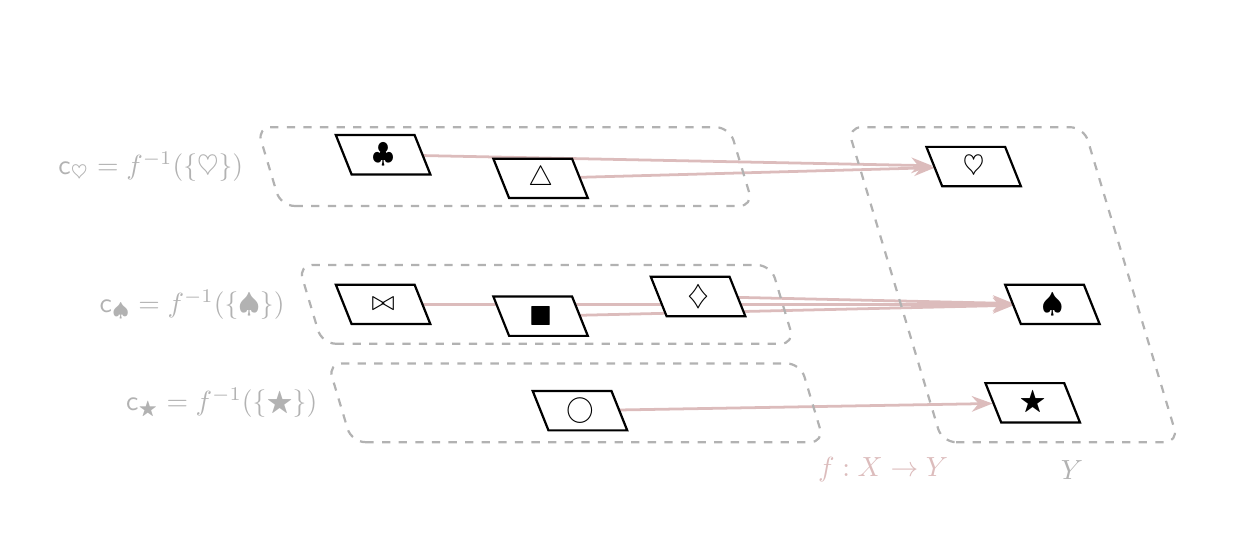
\begin{tikzpicture}[scale=1, thick]

  \draw[white] (-6.5, -3) rectangle (8.5, 3.25);
  
  \pgfmathsetmacro{\dx}{0.5}
  \pgfmathsetmacro{\dy}{0.25}
  \pgfmathsetmacro{\tilt}{0.2}
  
  \foreach \xi/\yi/\xf/\yf/\si/\sf in {0/-0.4/6.5/-0.25/0/14, -2/1.65/5.5/1.5/0/15, 2/-0.15/6.5/-0.25/0/14, 
                                       0.5/-1.6/6.25/-1.5/0/14.5, 0/1.35/5.5/1.5/0/14, -2/-0.25/6.5/-0.25/0/14} {
    \draw[light, -{Stealth}, line width=1, shorten <=\si, shorten >=\sf] (\xi, \yi) -- (\xf, \yf);                 
  }
  
  \foreach \x/\y\glyph [count=\n] in {0/-0.4/\blacksquare, -2/1.65/\clubsuit, 2/-0.15/\diamondsuit, 
                                      0.5/-1.6/\bigcirc, 0/1.35/\triangle, -2/-0.25/\bowtie} {
    \begin{scope}[shift={(\x, \y)}]
      \filldraw[fill=white, draw=black]    
           ({-(1 - \tilt) * \dx}, -\dy) -- ({(1 + \tilt) * \dx}, -\dy) 
        -- ({(1 - \tilt) * \dx}, \dy) -- ({-(1 + \tilt) * \dx}, \dy) -- cycle;
      \node at (0, 0) { $\glyph$ };
    \end{scope}
  }
  
  \pgfmathsetmacro{\Dx}{3}
  \pgfmathsetmacro{\Dy}{0.5}
  \pgfmathsetmacro{\tilt}{0.3 * \Dy / \Dx}
  \foreach \y/\glyph in {1.5/\heartsuit, -0.25/\spadesuit, -1.5/\bigstar} {
    \pgfmathsetmacro{\x}{-(1 - 0.7) * \y}
    \begin{scope}[shift={(\x, \y)}]
      \draw[gray70, dashed, rounded corners=5]    
           ({-(1 - \tilt) * \Dx}, -\Dy) -- ({+(1 + \tilt) * \Dx}, -\Dy) 
        -- ({+(1 - \tilt) * \Dx}, +\Dy) -- ({-(1 + \tilt) * \Dx}, +\Dy) -- cycle;
      \node[gray70] at (-1.5 * \Dx, 0) { $\mathsf{c}_{\glyph} = f^{-1}( \{ \glyph \} )$ };
    \end{scope}
  }
  
  \pgfmathsetmacro{\dx}{0.5}
  \pgfmathsetmacro{\dy}{0.25}
  \pgfmathsetmacro{\tilt}{0.2}
  \foreach \x/\y\glyph [count=\n] in {5.5/1.5/\heartsuit, 6.5/-0.25/\spadesuit, 6.25/-1.5/\bigstar } {
    \begin{scope}[shift={(\x, \y)}]
      \node at (0, 0) { $\glyph$ };
      \draw[black]    ({-(1 - \tilt) * \dx}, -\dy) -- ({(1 + \tilt) * \dx}, -\dy) 
                   -- ({(1 - \tilt) * \dx}, \dy) -- ({-(1 + \tilt) * \dx}, \dy) -- cycle;
    \end{scope}
  }
  
  \pgfmathsetmacro{\Dx}{1.5}
  \pgfmathsetmacro{\Dy}{2}
  \pgfmathsetmacro{\tilt}{0.3 * \Dy / \Dx}
    \begin{scope}[shift={(6, 0)}]
    \draw[gray70, dashed, rounded corners=5]    
         ({-(1 - \tilt) * \Dx}, -\Dy) -- ({(1 + \tilt) * \Dx}, -\Dy) 
      -- ({(1 - \tilt) * \Dx}, \Dy) -- ({-(1 + \tilt) * \Dx}, \Dy) -- cycle;
    \node[gray70] at (0.75, -2.35) { $Y$ };
  \end{scope}
  
  \node[light] at (4.35, -2.35) { $f : X \rightarrow Y$ };
\end{tikzpicture}

\end{document}  